\documentclass{beamer}

\newcommand{\course}{CS 1331 Introduction to Object Oriented Programming}
\newcommand{\lesson}{Swing, Part 3 of 5}
\newcommand{\code}{http://www.cc.gatech.edu/~simpkins/teaching/gatech/cs1331/code}

\author[Chris Simpkins] 
{Christopher Simpkins \\\texttt{chris.simpkins@gatech.edu}}
\institute[Georgia Tech] % (optional, but mostly needed)

\date[CS 1331]{}

\subject{\lesson}


% If you have a file called "university-logo-filename.xxx", where xxx
% is a graphic format that can be processed by latex or pdflatex,
% resp., then you can add a logo as follows:

% \pgfdeclareimage[width=0.6in]{coc-logo}{cc_2012_logo}
% \logo{\pgfuseimage{coc-logo}}

\mode<presentation>
{
  \usetheme{Berlin}
  \useoutertheme{infolines}

  % or ...

 \setbeamercovered{transparent}
  % or whatever (possibly just delete it)
}

\usepackage{hyperref}
\usepackage{fancybox}
\usepackage{listings}
\usepackage[abbr]{harvard}

\usepackage[english]{babel}
% or whatever

\usepackage[utf8]{inputenc}
% or whatever

\usepackage{times}
\usepackage[T1]{fontenc}
% Or whatever. Note that the encoding and the font should match. If T1
% does not look nice, try deleting the line with the fontenc.


\usepackage{listings}
 
% "define" Scala
\lstdefinelanguage{scala}{
  morekeywords={abstract,case,catch,class,def,%
    do,else,extends,false,final,finally,%
    for,if,implicit,import,match,mixin,%
    new,null,object,override,package,%
    private,protected,requires,return,sealed,%
    super,this,throw,trait,true,try,%
    type,val,var,while,with,yield},
  otherkeywords={=>,<-,<\%,<:,>:,\#,@},
  sensitive=true,
  morecomment=[l]{//},
  morecomment=[n]{/*}{*/},
  morestring=[b]",
  morestring=[b]',
  morestring=[b]""",
}

\usepackage{color}
\definecolor{dkgreen}{rgb}{0,0.6,0}
\definecolor{gray}{rgb}{0.5,0.5,0.5}
\definecolor{mauve}{rgb}{0.58,0,0.82}
 
% Default settings for code listings
\lstset{frame=tb,
  language=scala,
  aboveskip=2mm,
  belowskip=2mm,
  showstringspaces=false,
  columns=flexible,
  basicstyle={\scriptsize\ttfamily},
  numbers=none,
  numberstyle=\tiny\color{gray},
  keywordstyle=\color{blue},
  commentstyle=\color{dkgreen},
  stringstyle=\color{mauve},
  frame=single,
  breaklines=true,
  breakatwhitespace=true,
  keepspaces=true
  %tabsize=3
}


\title[\course] % (optional, use only with long
                                      % paper titles)
{\lesson}

\subtitle{}
%% {Include Only If Paper Has a Subtitle}

\newcommand{\link}[2]{\href{#1}{\textcolor{blue}{\underline{#2}}}}


% If you wish to uncover everything in a step-wise fashion, uncomment
% the following command: 

% \beamerdefaultoverlayspecification{<+->}


\begin{document}

\begin{frame}
  \titlepage
\end{frame}

%------------------------------------------------------------------------
\begin{frame}[fragile]{Outline}


\begin{itemize}
\item Listeners and Inner Classes
\item Actions
\item Lists, ListModels and the MVC Pattern
\item General Structure of Swing Hierarchy
\item ScrollPanes and the Decorator Pattern
\item Dialog Boxes
\end{itemize}


\end{frame}
%------------------------------------------------------------------------

%------------------------------------------------------------------------
\begin{frame}[fragile]{Inner Classes}


We've defined our listeners as public top-level classes, but if they're only used in one class they can be defined within the class that uses them:

\begin{lstlisting}[language=Java]
public class CompanyFrame extends JFrame {

    private class NewEmpListener implements ActionListener {
        public void actionPerformed(ActionEvent e) { ... }
    }
// ...
\end{lstlisting}

And instantiated where needed:

\begin{lstlisting}[language=Java]
JButton newEmpButton = new JButton("New Employee...");
newEmpButton.addActionListener(new NewEmpListener());
\end{lstlisting}


\end{frame}
%------------------------------------------------------------------------

%------------------------------------------------------------------------
\begin{frame}[fragile]{Anonymous Inner Classes}


If an inner class is used only once, we can define it and instantiate an instance of it anonymously at the same time:
\begin{lstlisting}[language=Java]
newEmpButton.addActionListener(new ActionListener() {
    public void actionPerformed(ActionEvent e) {
        System.out.println("New button.  It was clicked.");
    }
});
\end{lstlisting}

\begin{itemize}
\item The syntax {\tt new ActionListener() \{ ... \}} means ``instantiate an instance of a class that's a subclass of {\tt ActionListener}'.'
\item Required method definitions are given between {\tt \{ ... \}}.
\end{itemize}

You'll see this idiom a lot in Swing code.


\end{frame}
%------------------------------------------------------------------------

%------------------------------------------------------------------------
\begin{frame}[fragile]{The Model-View-Controller Design Pattern}
\vspace{-.1in}
\begin{center}
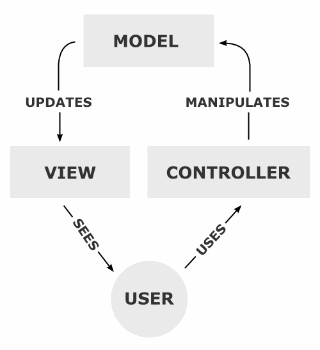
\includegraphics[height=1.5in]{MVC-Process.png}\footnote{\url{http://en.wikipedia.org/wiki/File:MVC-Process.png}}
\end{center}
\vspace{-.1in}
\begin{itemize}
\item The {\it model} contains the data that is displayed by the {\it view}
\item The {\it view} displays the data from the {\it model} on screen
\item The {\it controller} gets input from the user and manipulates the model
\end{itemize}
In Swing the view and controller are often combined.

\end{frame}
%------------------------------------------------------------------------

%------------------------------------------------------------------------
\begin{frame}[fragile]{{\tt JList}, {\tt ListModel}, and MVC}


Our main application Frame, {\tt CompanyFrame} takes a {\tt ListModel} as an argument:
\begin{lstlisting}[language=Java]
public CompanyFrame(ListModel employeeListModel) {
    // ...
    add(new JList(employeeListModel), BorderLayout.CENTER);
    // ...
}
\end{lstlisting}
And we build the {\tt ListModel} before we show the main application frame:
\begin{lstlisting}[language=Java]
Company company = new Company(file);
DefaultListModel lm = new DefaultListModel();
for (Employee e: company.getEmployees()) {
    lm.addElement(e);
}
CompanyFrame cf = new CompanyFrame(lm);  
\end{lstlisting}


\end{frame}
%------------------------------------------------------------------------

%------------------------------------------------------------------------
\begin{frame}[fragile]{General Structure of Swing Hierarchy}


{\tt ListModel} and its descendant classes are typical of the structure of many Swing classes:
\begin{center}
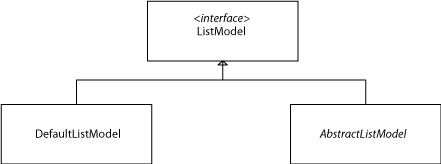
\includegraphics[height=1.5in]{list-model-hierarchy.png}
\end{center}

\begin{itemize}
\item {\tt ListModel} is the general interface
\item {\tt DefaultListModel} is a ready-to-use implementation for simple cases.
\item {\tt AbstractListModel} is a class that can be built upon for complex needs.
\end{itemize}


\end{frame}
%------------------------------------------------------------------------

%------------------------------------------------------------------------
\begin{frame}[fragile]{The Decorator Design Pattern}


{\bf The Decorator Pattern}\footnote{Gamma, Helms, Johns, and Vlissides, {\it Design Patterns: Elements of Reusable Object-Oriented Software}, Addison-Wesley, 1994}\\
Attach additional responsibilities to an object dynamically. Decorators provide a flexible alternative to subclassing for extending functionality.\\

\begin{center}
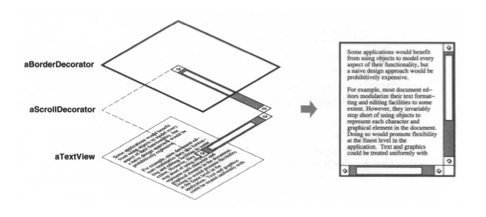
\includegraphics[height=1.75in]{gof-decorator-diagram.png}
\end{center}



\end{frame}
%------------------------------------------------------------------------

%------------------------------------------------------------------------
\begin{frame}[fragile]{{\tt JScrollPane} and the Decorator Pattern}


The Swing l ibrary provides a scrollbar decorator called {\tt JScrollPane}.  Using it is easy:
\begin{lstlisting}[language=Java]
add(new JScrollPane(new JList(employeeListModel)), BorderLayout.CENTER);
\end{lstlisting}
By simply wrapping our {\tt JList} in a {\tt JScrollPane} the list will show horizontal and vertical scroll bars as needed.

\begin{center}
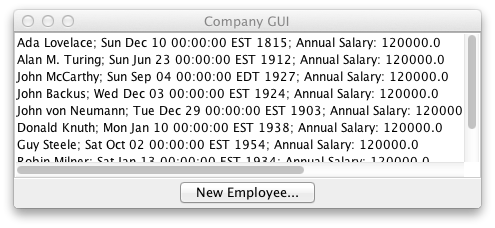
\includegraphics[height=1.75in]{CompanyGui.png}
\end{center}


\end{frame}
%------------------------------------------------------------------------

%------------------------------------------------------------------------
\begin{frame}[fragile]{Dialog Windows}


A dialog window:
\begin{itemize}
\item is an independent subwindow that conveys information or gets input form the user.
\item can be {\it modal}, meaning that the dialog window blocks its parent {\tt Frame} while the dialog is visible, or {\it modeless} meaning it does not block its parent window. 
\end{itemize}
In Swing:
\begin{itemize}
\item Every dialog is dependent on a Frame.  When a dialog's parent Frame is destroyed, so is the dialog.
\item Simple modal dialogs can be created easily with {\tt JOptionPane}.
\item Custom dialogs can be created by extending {\tt JDialog}.
\end{itemize}

We'll see examples of both.

\end{frame}
%------------------------------------------------------------------------

%------------------------------------------------------------------------
\begin{frame}[fragile]{Simple Dialogs with {\tt JOptionPane}}


{\tt JOptionPane} has several static methods that instantiate and display simple dialogs.  The most common are (from the Java API):

\begin{itemize}
\item {\tt showConfirmDialog} asks a confirming question, like yes/no/cancel.
\item {\tt showInputDialog} prompts prompts the user for input.
\item {\tt showMessageDialog} displays a message to the user.
\item {\tt showOptionDialog} is The Grand Unification of the above three.
\end{itemize}
For example, the line:
\begin{lstlisting}[language=Java]
JOptionPane.showMessageDialog(null, "Simple message.");
\end{lstlisting}
\begin{columns}[c]
\begin{column}{2in}
displays the dialog:
\end{column}
\begin{column}{2in}
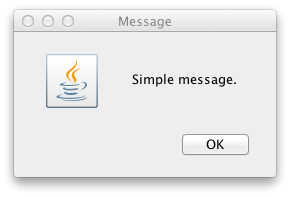
\includegraphics[height=1in]{simple-message-dialog.png}
\end{column}
\end{columns}

\end{frame}
%------------------------------------------------------------------------

%------------------------------------------------------------------------
\begin{frame}[fragile]{Custom Dialogs with {\tt JDialog}}


To create a custom dialog, extend {\tt JDialog}.  Custom dialogs require consideration of

\begin{itemize}
\item Modality - should the dialog be modal or modeless?
\item Visual design - a dialog box is a visual component just like any other GUI component.
\item UI design:
\begin{itemize}
\item Make it clear how the dialog box fits into the overall GUI application (how it is launched, what happens if the user clicks OK or Cancel).
\item Make it clear what the user is expected to do with the dialog.
\item Give the user useful error messages if they do something wrong.
\end{itemize}
\end{itemize}

Let's look at some examples in the \link{\code/swing/companygui/}{Company GUI} (particularly \link{\code/swing/companygui/SalariedEmployeeDialog.java}{SalariedEmployeeDialog.java} and \link{\code/swing/companygui/HourlyEmployeeDialog.java}{HourlyEmployeeDialog.java}.

\end{frame}
%------------------------------------------------------------------------


% %------------------------------------------------------------------------
% \begin{frame}[fragile]{}


% \begin{lstlisting}[language=Java]

% \end{lstlisting}

% \begin{itemize}
% \item
% \end{itemize}


% \end{frame}
% %------------------------------------------------------------------------


\end{document}
